%%%%%%%%%%%%%%%%%%%%%%%%%%%%%%%%%%%%%%%%%%%%%%%%%%%%%%%%%%%%%%%%%%%%%%%%%%%%%%%%
% > Лабораторная работа 4: Крутильные колебания вала с дисками.
% > Баталов Семен, Антонова Мария, Клюшин Максим, Хайретдинова Диана.
% > 2021 год.
%%%%%%%%%%%%%%%%%%%%%%%%%%%%%%%%%%%%%%%%%%%%%%%%%%%%%%%%%%%%%%%%%%%%%%%%%%%%%%%%

\documentclass[12pt, a4paper]{article}
\usepackage[left=2cm, right=2cm, top=2.5cm, bottom=2.5cm, nohead, 
footskip=1cm]{geometry}
\usepackage{graphicx}
\graphicspath{{./Pictures/}}
\usepackage[utf8]{inputenc}
\usepackage[english, russian]{babel}
\usepackage{indentfirst}
\usepackage{array}
\usepackage{longtable}
\usepackage{misccorr}
\usepackage{setspace, amsmath}
\usepackage{multirow}

\begin{document}
    
    \newcolumntype{M}[1]{>{\centering\arraybackslash}m{#1}}
    \renewcommand{\arraystretch}{1.4}
    
    \begin{center}
        \large{Санкт-Петербургский государственный университет} \\
        \large{Saint-Petersburg State University}\\
        \hfill \break
        \hfill \break
        \hfill \break
        \hfill \break
        \hfill \break
        \hfill \break
        \hfill \break
        \large{Кафедра теоретической и прикладной механики} \\
        \hfill \break
        \hfill \break
        \large{\textbf{ОТЧЕТ}} \\
        \large{\textbf{По лабораторной работе 4}} \\
        \large{<<Крутильные колебания вала с дисками>>} \\
        \hfill \break
        \hfill \break
        \hfill \break
        \large{По дисциплине} \\
        \large{<<Лабораторный практикум по теоретической механике>>} \\
    \end{center}
    
    \hfill \break
    \hfill \break
    \hfill \break
    \hfill \break
    \hfill \break
    \hfill \break
    
    \begin{flushright} 
        \large{Выполнили:} \\
        \hfill \break
        \large{Баталов С. А.} \\
        \large{Антонова М. } \\
        \large{Клюшин М.} \\
        \large{Хайретдинова Д.} \\
    \end{flushright}
    
    \hfill \break
    \hfill \break
    \hfill \break
    \hfill \break
    
    \begin{center} 
        \large{Санкт-Петербург} \\
        \large{2021} \\
    \end{center}
    
    \thispagestyle{empty}
    \newpage
    
    \section{Описание установки}
    
    В данной работе рассматриваются колебания механической системы с тремя степенями свободы. Целью работы является экспериментальное определение частот и главных форм собственных колебаний системы, их теоретический расчет и последующее сравнение.
    
    \begin{figure} [h]
        \centering
        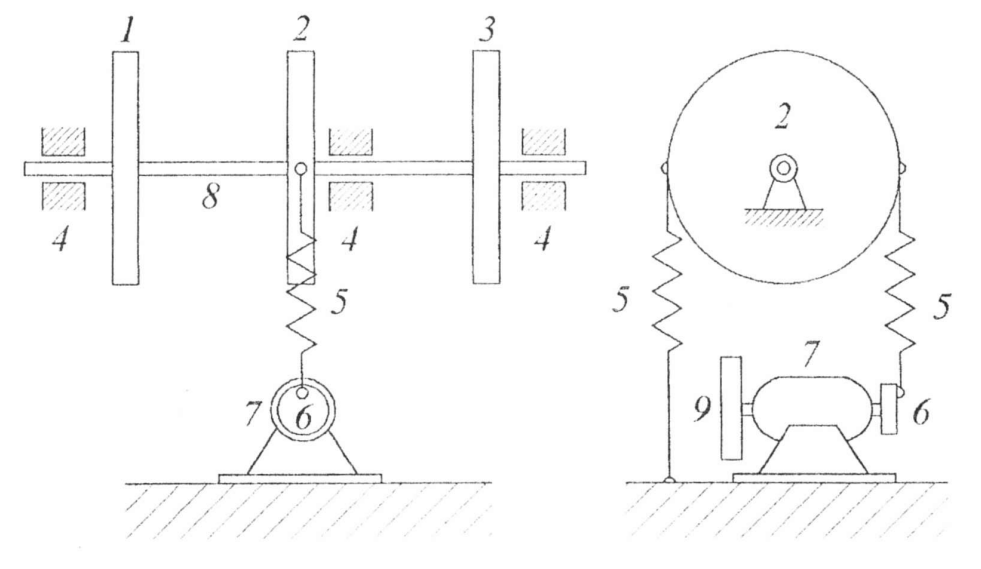
\includegraphics [width = 12cm] {Lab_4_1.png}
        \caption{\centering Схема лабораторной установки.}
        \label{im1}
    \end{figure}
    
    На рис.~\ref{im1} изображена схема лабораторной установки. Основной частью установки является упругий вал \textit{8} с тремя жестко укрепленными на нем дисками \textit{1}, \textit{2} и \textit{3}. Вал может вращаться в подшипниках \textit{4}, установленных на станине. К ободу среднего диска \textit{2} прикреплены пружины \textit{5}, одна из которых связана со станиной, а другая~--~с эксцентриком \textit{6}, закрепленном на валу электродвигателя \textit{7}. На валу электродвигателя укреплены маховик \textit{9} для стабилизации частоты вращения и диск оптоэлектронного тахометрического датчика. Сигнал с тахометрического датчика поступает на вход электронного цифрового тахометра, показания которого соответствуют частоте вращения вала в герцах.
    
    \newpage
    
    \section{Параметры установки}
    
    В следующей таблице представлены заранее известные величины: плотность материала дисков~--~$\rho$, модуль сдвига материала вала~--~$G$, жесткость пружины~--~$c_{\text{п}}$.
    
    \begin{longtable}{| M{2cm} | M{3cm} | M{3cm} | M{3cm} |}
        \caption{\centering Известные константы.}
        \label{tb1} \\
        \hline
        Номер & Величина & Значение & Размерность \\
        \hline
        1 & $\rho$ & $7,85 \cdot 10^{3}$ & $\text{кг} / \text{м}^{3}$ \\
        \hline
        2 & $G$ & $8,33 \cdot 10^{10}$ & Па \\
        \hline
        3 & $c_{\text{п}}$ & 4900 & $\text{Н} / \text{м}$ \\
        \hline
    \end{longtable}
    
    Для расчета частот и форм собственных колебаний системы потребуется измерить некоторые параметры установки. Данные измерений приведены в таблице \ref{tb2}. Здесь $r_{i}$~--~радиусы дисков, $d_{i}$~--~толщины дисков, $l_{i}$~--~расстояния между дисками, $r$~--~радиус упругого вала, $e$~--~расстояние от точки крепления пружины до центра эксцентрика.
    
    \begin{longtable}{| M{2cm} | M{3cm} | M{3cm} | M{3cm} | M{3cm} |}
        \caption{\centering Результаты измерений параметров установки.}
        \label{tb2} \\
        \hline
        Номер & Величина & Значение & Погрешность & Размерность \\
        \hline
        1 & $r_{1}$ & 0,150 & 0,0005 & м \\
        2 & $r_{2}$ & 0,150 & 0,0005 & м \\
        3 & $r_{3}$ & 0,150 & 0,0005 & м \\
        \hline
        4 & $d_{1}$ & 0,025 & 0,0005 & м \\
        5 & $d_{2}$ & 0,020 & 0,0005 & м \\
        6 & $d_{3}$ & 0,025 & 0,0005 & м \\
        \hline
        7 & $l_{1}$ & 0,445 & 0,0005 & м \\
        8 & $l_{2}$ & 0,616 & 0,0005 & м \\
        \hline
        9 & $r$ & 0,005 & 0,00005 & м \\
        \hline
        10 & $e$ & 0,021 & 0,0005 & м \\
        \hline
    \end{longtable}
    
    \newpage
    
    \section{Теоретические исследования}
    
    Для начала произведем вспомогательные вычисления и расчитаем моменты инерции дисков. Для этого воспользуемся формулой~(\ref{eq1}).
    
    \begin{equation}
        I_{i} = \frac{1}{2} m_{i} r_{i}^{2} = \frac{1}{2} \rho \pi r_{i}^{4} d_{i}, \quad
        i = 1, \, 2, \, 3.
        \label{eq1}
    \end{equation}
    
    Далее определим жесткость на скручивание участков вала. Воспользуемся формулой~(\ref{eq2}). Здесь $I_{p} = \frac{1}{2} \pi r^{4}$~--~полярный момент инерции поперечного сечения вала.
    
    \begin{equation}
        c_{k} = \frac{G I_{p}}{l_{k}} = \frac{G \pi r^{4}}{2 l_{k}}, \quad
        k = 1, \, 2.
        \label{eq2}
    \end{equation}
    
    Для дальнейшей работы составляется система уравнений Лагранжа второго рода для данной задачи и упрощается. В итоге приходим к уравнению (\ref{eq3}), решениями которого являются квадраты искомых частот $\omega_{i}$ собственных колебаний системы.
    
    \begin{equation}
        a_{0}y^{3} + a_{1}y^{2} + a_{2}y + a_{3} = 0, \quad
        y = \omega^{2}.
        \label{eq3}
    \end{equation}
    
    Здесь
    
    \begin{gather*}
        a_{0} = I_{1} I_{2} I_{3}, \quad
        a_{1} = -c_{2} I_{1} I_{2} - c_{3} I_{1} I_{3} - c_{1} I_{2} I_{3}, \\
        a_{2} = c_{2} (c_{3} - c_{2}) I_{1} + c_{1} c_{2} I_{2} + c_{1} (c_{3} - c_{1}) I_{3}, \\
        a_{3} = -c_{1} c_{2} (c_{3} - c_{1} - c_{2}), \quad
        c_{3} = c_{1} + c_{2} + 2 c_{\text{п}} r_{2}^{2}.
    \end{gather*}
    
    Для поиска главных форм собственных колебаний воспользуемся формулами (\ref{eq4}) и (\ref{eq5}). Найти значения амплитуд $\Phi_{i}(\omega)$ колебаний дисков можно с помощью выражения (\ref{eq5}). Отношение амплитуд при резонансе можно расчитать по формуле (\ref{eq6}).
    
    \begin{equation}
        \Delta(\omega) = 
        \begin{vmatrix}
            c_{1} - \omega^{2} I_{1} & -c_{1} & 0 \\
            -c_{1} & c_{3} - \omega^{2} I_{2} & -c_{2} \\
            0 & -c_{2} & c_{2} - \omega^{2} I_{3} \\
        \end{vmatrix}, \qquad
        b = 
        \begin{pmatrix}
            0 \\
            r_{2} c_{\text{п}} e \\
            0 \\
        \end{pmatrix}.
        \label{eq4}
    \end{equation}
    
    Далее используется обозначение $\Delta_{i}(\omega)$~--~определитель, полученный из определителя $\Delta(\omega)$ заменой $i$-го столбца столбцом свободных членов $b$.
    
    \begin{equation}
        \Phi_{i}(\omega) = \frac{\Delta_{i}(\omega)}{\Delta(\omega)}, \quad
        i = 1, \, 2, \, 3.
        \label{eq5}
    \end{equation}
    
    \begin{equation}
        \frac{\Phi_{1}(\omega_{k})}{\Phi_{2}(\omega_{k})} = \frac{\Delta_{1}(\omega_{k})}{\Delta_{2}(\omega_{k})}, \quad
        \frac{\Phi_{2}(\omega_{k})}{\Phi_{3}(\omega_{k})} = \frac{\Delta_{2}(\omega_{k})}{\Delta_{3}(\omega_{k})}, \quad
        k = 1, \, 2, \, 3.
        \label{eq6}
    \end{equation}
    
    \newpage
    
    \section{Результаты расчетов}
    
    \begin{longtable}{| M{2cm} | M{3cm} | M{3cm} | M{3cm} |}
        \caption{\centering Расчет вспомогательных величин.}
        \label{tb3} \\
        \hline
        Номер & Величина & Значение & Размерность \\
        \hline
        1 & $I_{1}$ & 0,1561 & $\text{кг} \cdot \text{м}^{2}$ \\
        2 & $I_{2}$ & 0,1249 & $\text{кг} \cdot \text{м}^{2}$ \\
        3 & $I_{3}$ & 0,1561 & $\text{кг} \cdot \text{м}^{2}$ \\
        \hline
        4 & $c_{1}$ & 183,7743 & $\text{Н} \cdot \text{м}$ \\
        5 & $c_{2}$ & 132,7591 & $\text{Н} \cdot \text{м}$ \\
        6 & $c_{3}$ & 537,0334 & $\text{Н} \cdot \text{м}$ \\
        \hline
    \end{longtable}
    
    \begin{longtable}{| M{2cm} | M{3cm} | M{3cm} |}
        \caption{\centering Расчет коэффициентов уравнения (\ref{eq3}).}
        \label{tb4} \\
        \hline
        Номер & Величина & Значение \\
        \hline
        1 & $a_{0}$ & 0,0030 \\
        2 & $a_{1}$ & -19,2574 \\
        3 & $a_{2}$ & 21559,3348 \\
        4 & $a_{3}$ & -5379695,2030 \\
        \hline
    \end{longtable}
    
    \begin{longtable}{| M{2cm} | M{3cm} | M{3cm} |}
        \caption{\centering Расчет определителей.}
        \label{tb5} \\
        \hline
        Номер & Величина & Значение \\
        \hline
        1 & $\Delta_{1}(\omega_{1})$ &  \\
        2 & $\Delta_{2}(\omega_{1})$ &  \\
        3 & $\Delta_{3}(\omega_{1})$ &  \\
        \hline
        4 & $\Delta_{1}(\omega_{2})$ &  \\
        5 & $\Delta_{2}(\omega_{2})$ &  \\
        6 & $\Delta_{3}(\omega_{2})$ &  \\
        \hline
        7 & $\Delta_{1}(\omega_{3})$ &  \\
        8 & $\Delta_{2}(\omega_{3})$ &  \\
        9 & $\Delta_{3}(\omega_{3})$ &  \\
        \hline
    \end{longtable}
    
    \begin{longtable}{| M{2cm} | M{3cm} | M{3cm} | M{3cm} |}
        \caption{\centering Собственные частоты и формы колебаний системы.}
        \label{tb6} \\
        \hline
        Номер & Величина & Значение & Размерность \\
        \hline
        1 & $\omega_{1}$ & 18,90 & $1 / \text{с}$ \\
        2 & $\omega_{2}$ & 31,47 & $1 / \text{с}$ \\
        3 & $\omega_{3}$ & 71,22 & $1 / \text{с}$ \\
        \hline
        4 & $\Phi_{1}(\omega_{1})$ &  & -- \\
        5 & $\Phi_{2}(\omega_{1})$ &  & -- \\
        6 & $\Phi_{3}(\omega_{1})$ &  & -- \\
        \hline
        7 & $\Phi_{1}(\omega_{2})$ &  & -- \\
        8 & $\Phi_{2}(\omega_{2})$ &  & -- \\
        9 & $\Phi_{3}(\omega_{2})$ &  & -- \\
        \hline
        10 & $\Phi_{1}(\omega_{3})$ &  & -- \\
        11 & $\Phi_{2}(\omega_{3})$ &  & -- \\
        12 & $\Phi_{3}(\omega_{3})$ &  & -- \\
        \hline
    \end{longtable}
    
    \newpage
    
    \section{Результаты экспериментов}
    
    \begin{longtable}{| M{2cm} | M{3cm} | M{3cm} | M{3cm} | M{3cm} |}
        \caption{\centering Экспериментальные значения частот собственных колебаний системы.}
        \label{tb7} \\
        \hline
        \multirow{2}{*}{Номер} &
        \multirow{2}{*}{Величина} &
        \multicolumn{2}{M{6cm}|}{Значение} &
        \multirow{2}{*}{Размерность} \\
        \cline{3-4}
        & & Теория & Эксперимент & \\
        \hline
        1 & $\omega_{1}$ & 18,90 &  & $1 / \text{с}$ \\
        2 & $\omega_{2}$ & 31,47 &  & $1 / \text{с}$ \\
        3 & $\omega_{3}$ & 71,22 &  & $1 / \text{с}$ \\
        \hline
    \end{longtable}
    
    \newpage
    
    \section{Выводы}
    
\end{document}